%----------------------------------------------------------
%
\documentclass[xcolor=dvipsnames]{beamer}%

\mode<presentation> {
  \usetheme{CambridgeUS}
  \usefonttheme[onlymath]{serif}
  \setbeamercovered{transparent}
}

\usepackage{hyperref}

\hypersetup{colorlinks,linkcolor=,urlcolor=blue}
\usepackage{minted}
\usepackage{multicol}
%\usepackage{utf-8}

\setbeamertemplate{itemize item}{\raisebox{0.25ex}{\small\textbullet}}
\setbeamertemplate{itemize subitem}{\raisebox{0.25ex}{\scriptsize\textbullet}}
\graphicspath{{figures/}}
\logo{\resizebox{10mm}{!}{\includegraphics{fer_logo.jpg}}}
\setbeamersize{text margin left=15pt, text margin right=20pt} 
\setlength{\leftmarginii}{10pt}
\setbeamertemplate{enumerate item}{
    \raisebox{-1.7pt}{\scalebox{2.1}{\textbullet}\hskip-14.3pt}
    \hbox to2ex{%
      \hfil
      \usebeamercolor[bg]{item projected}
      \color{fg}
      \raisebox{1.7pt}{\scalebox{0.65}{\insertenumlabel}}%
      \hfil}
    \hskip-5pt%
}
\setbeamertemplate{section in toc}{
  \leavevmode\leftskip=3ex%
  \llap{%
    \usebeamerfont*{section number projected}%
    \usebeamercolor{section number projected}%
    \begin{pgfpicture}{-1ex}{-0.3ex}{1ex}{2ex}
      \color{bg}
      \pgfpathcircle{\pgfpoint{0pt}{.75ex}}{1.7ex}
      \pgfusepath{fill}
      \pgftext[base]{\color{fg}\inserttocsectionnumber}
    \end{pgfpicture}\kern2.25ex%
  }%
  \inserttocsection\par}
\setbeamertemplate{subsection in toc}
  {\leavevmode\leftskip=2em$\bullet$\hskip1em\inserttocsubsection\par}

%------------------------------------------------------------------

%%% --------------------------------------------------------------
\title[git basics]
{LARICS git tutorial}

\author[Or\v{s}uli\'{c}, Mikli\'{c}]{Juraj Or\v{s}uli\'{c}, Damjan Mikli\'{c}}

\institute[LARICS]{LARICS Lab\\FER, University of Zagreb}

\date[]{December 2018}

%\AtBeginSection[]
%{
%  \begin{frame}<beamer>{Outline}
%    \tableofcontents[currentsection]
%  \end{frame}
%}

\begin{document}
% ================================================================

\begin{frame}
	\titlepage
\end{frame}

% ----------------------------------------------------------------
\section*{Outline}
\begin {frame}
	\tableofcontents
\end{frame}


% =============================================================================

\section{Preparation}

\begin{frame}[fragile]

\frametitle{A note on notation}
	
Throughout the presentation, the following notation applies:

\begin{itemize}
	\item Commands that you are supposed to type are displayed in \texttt{monospace font} preceded by a \texttt{>} symbol, such as
	\begin{minted}{console}
> git --help
	\end{minted}
	\item The \texttt{>} symbol only indicates the command prompt.\\ \textit{Do not} type it in.
	\item When the command is too long to fit in one line, the line break will be escaped with a backslash (\textbackslash). You do not need to type in the backslash and the line break.
	\item The text that you need to replace is given \texttt{<inside angle brackets>}, e.g.,
	\begin{minted}{console}
> cd /home/<your username>
	\end{minted}
	When typing in the command with your replaced text, omit \\the brackets.
\end{itemize}

\end{frame}

% -----------------------------------------------------------------------------

\begin{frame}[fragile]

\frametitle{Preparing for the tutorial}
	
\begin{itemize}
	\item  Open a \href{https://github.com/join?source=header-home}{GitHub account} and set up an SSH key for passwordless login according to \href{https://help.github.com/articles/adding-a-new-ssh-key-to-your-github-account/}{these instructions on Github}
	\item Install the git command-line client and GUI tools
	\begin{minted}{console}
> sudo apt install git git-gui gitg
	\end{minted}
	\item Tell git who you are, and which editor to use:
	\begin{minted}{console}
> git config --global user.name "<Your Name>"
> git config --global user.email <youremail@fer.hr>
> git config --global core.editor \
  "gedit --wait --new-window"
	\end{minted}
	\item The code example in the exercise will be available in C++ and Python. If you will be using C++, install the build tools:
	\begin{minted}{console}
> sudo apt install build-essential cmake
	\end{minted}
\end{itemize}

\end{frame}

% -----------------------------------------------------------------------------

\begin{frame}

\frametitle{Tutorial organization}
	
\begin{itemize}
	\item Work in pairs
	\item Pair up with someone using the same programming language (C++ or Python)
	\item When assigning tasks and describing how you will interact with each other through git, we will refer to you, the members of a pair, as \textit{Mirko} and \textit{Slavko}. Make an agreement about who will assume each role.
\end{itemize}
	
\end{frame}

% -----------------------------------------------------------------------------


% =============================================================================

\section{The basic basics}

\begin{frame}

\frametitle{Version control system}
	
	\begin{itemize}
	\item \emph{VCS} - version control system
	\end{itemize}
	
\begin{block}{Basic features}
	\begin{itemize}
		\item Keeps track of changes to our code
		\item Facilitates collaboration in software and documentation development
	\end{itemize}
\end{block}
	
\begin{block}{Additional requirements}
	\begin{itemize}
		\item Work offline
		\item Support a distributed, decentralized workflow
		\item Compatibility with existing protocols (e.g. ssh, http)
		\item Data integrity protection
		\item Efficiency
	\end{itemize}
\end{block}

\end{frame}

% -----------------------------------------------------------------------------

\begin{frame}

\frametitle{About git}
	
\begin{itemize}
	\item Developed in 2005 by Linus Torvalds (in a single weekend!) to support Linux kernel development
	\item Very powerful, has a reputation of being hard to learn
	\begin{itemize}
	\item We hope we will convince you otherwise :)
	\end{itemize}
	\item Supports different workflows
	\begin{itemize}
	\item We'll be using the GitHub workflow (more or less)	
	\end{itemize}
\end{itemize}

\begin{block}{Meaning of the name \emph{git}}
\small
\emph{git} means "unpleasant person" in British slang. Linus: "I'm an egotistical bastard, and I name all my projects after myself."

\medskip
From the readme:
	 \begin{itemize}
	 \item "global information tracker": you're in a good mood, and it actually works for you. Angels sing, and a light suddenly fills the room.
	 \item "g*dd*mn idiotic truckload of sh*t": when it breaks
	 \end{itemize}
	 
\end{block}

\end{frame}

% -----------------------------------------------------------------------------

\begin{frame}

\frametitle{Basic terms: repository and commit}
\begin{block}{Repository (repo)}
	A place where your work is kept. It contains your code and its complete history, stored as a collection of commits.
\end{block}

\begin{block}{Commit}
	A basic unit of work in a project. Contains the set of changes, a textual description of what these changes do, a reference to the previous state (the \textit{parent commit}), and the author name and date.\\ \smallskip Finally, the commit contains an alphanumeric identifier (SHA-1 hash), generated from the above information, which is used to uniquely identify the commit. \\For example: \textcolor{Maroon}{\texttt{bdfa760c07d8f621ff603a2dc5d6de810cd62e88}}
\smallskip

You can also use a prefix of the identifier to refer to this commit, usually 5 or 7 characters long, e.g. \textcolor{Maroon}{\texttt{bdfa760}}.
\end{block}
\end{frame}

% -----------------------------------------------------------------------------

\begin{frame}

\frametitle{Basic terms: branch, master and head}

\begin{block}{Branch, master and head}
A \alert{branch} is simply a pointer to a commit. \alert{Master} is the name of the default branch. \alert{Head} is a pointer to the last commit in the currently active (checked out) branch.
\end{block}

\begin{figure}
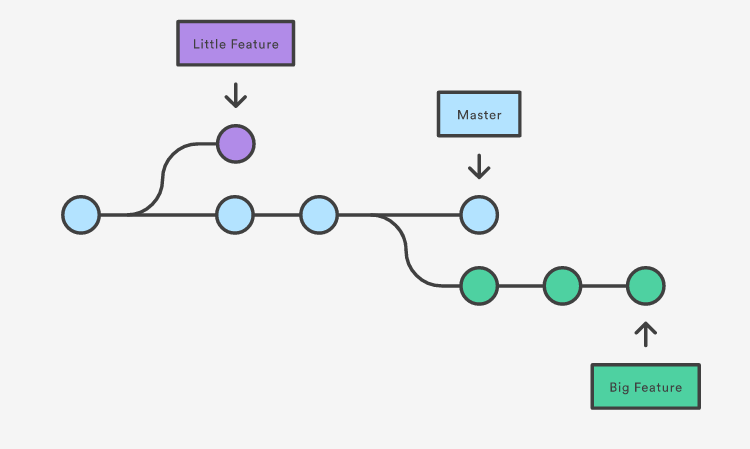
\includegraphics[scale=0.3]{branches}
\end{figure}

\end{frame}

% -----------------------------------------------------------------------------

\begin{frame}

\frametitle{Getting started on Github}

To begin working on a project using Github, you have to create a repository. There are two ways to do this:


\begin{itemize}
	\item Create an empty repository
	\begin{itemize}
	\item When starting from scratch
	\end{itemize}	
	
	\medskip
	\item Fork another repository
	\begin{itemize}
	\item When you wish to improve and build upon another repository
	\item This creates your personal copy of the repository in which you can make your own commits
	\end{itemize}
\end{itemize}

\end{frame}

% -----------------------------------------------------------------------------

\begin{frame}[fragile]

\frametitle{Making a Github fork and adding a collaborator}

\begin{block}{Task A [Mirko]: Fork the example repository}

	To fork a repository, simply click the \includegraphics[scale=0.35]{fork} \, icon in the top right corner of the repository webpage. For this tutorial, you will need to fork the \href{https://github.com/larics/git-tutorial-code.git}{larics/git-tutorial-code} repository.
\end{block}

\begin{block}{Task B [Mirko]: Add a collaborator to your forked repository}
In the GitHub user interface, on the \includegraphics[scale=0.35]{settings} \, tab of your forked repository, select the \texttt{Collaborators and teams} menu and add your partner as a collaborator with \texttt{Write} access.
\end{block}

\begin{block}{Task C [Slavko]: Accept the collaboration invitation}
Check your mail, or the list of notifications on Github. Accept the collaboration invitation.
\end{block}

\end{frame}

% -----------------------------------------------------------------------------

\begin{frame}[fragile]

\frametitle{Cloning the repository}

\begin{block}{Cloning}
Cloning creates a local copy of the repository, which includes all the commits in the repository -- the whole history.
\begin{minted}{console}
> git clone git@github.com:<you>/git-tutorial-code.git
\end{minted}
\end{block}

\begin{block}{Task D [Mirko, Slavko]}
Clone Mirko's repository onto your computer.
\end{block}

	
\end{frame}

% -----------------------------------------------------------------------------

\begin{frame}[fragile]

\frametitle{Repository structure}

What is contained in the repository directory?
	
\begin{minted}{console}
> cd git-tutorial-code
> ls -la
> git status
\end{minted}
	
\begin{itemize}
	\item The \textit{working tree} -- current version of files ("checked out")
	\item The hidden \texttt{.git} folder which contains repository metadata \\ (all the commits, and the internal structures for storing them)
	\item The \texttt{git status} command provides an overview of what is going on in the git repository.
\end{itemize}
\begin{minted}{console}
\end{minted}
	
\end{frame}

% -----------------------------------------------------------------------------

\begin{frame}
	\frametitle{Visualizing git operation}
	
	\begin{figure}
		\includegraphics[scale=0.4]{git-transport}
	\end{figure}
\end{frame}

% -----------------------------------------------------------------------------


\begin{frame}[fragile]
	\frametitle{Your first commit}
	
	\begin{block}{Task E [Mirko, Slavko]}
	Open \texttt{README.md} and add the following lines, then save the file:
	\begin{minted}{text}
Maintainers:
  <your name>
	\end{minted}

Run the following, and observe what is happening.

	\begin{minted}{console}
> git status
> git diff
> git add README.md
> git status
> git gui
> git commit -m "Add maintainer."
> git status
> git log
	\end{minted}
	
	\end{block}
	
\end{frame}

% -----------------------------------------------------------------------------


\begin{frame}[fragile]

\frametitle{Making a commit - recap}
	
\begin{enumerate}
	\item Make a change in the working tree. For example:
	\begin{itemize}
	\item Edit a file
	\item Create a file
	\item Delete a file 
	\item Move a file (git considers moving as deleting + creating a new file)
	\end{itemize}
	\item \texttt {git add} the change to the \textit{staging area} ("index")
	\item Perform a final inspection of the staged changes
	\begin{itemize}
	\item \texttt{git gui} is handy for this
	\item The staged changes should make a logically grouped set of changes
	\item Feel free to make as many commits as you like
	\item "Commit early and often"
	\end{itemize}
	\item \texttt{git commit} your changes
	\begin{itemize}
	\item  "50/72" rule - the title of the commit description should be {\raise.17ex\hbox{$\scriptstyle\sim$}}50 characters, the body should be wrapped to 72 characters
	\item Use the imperative form as the first word in the title -- e.g. \\"Add prime checking", "Implement saving to file", "Fix broken build"
	\end{itemize}
\end{enumerate}
	
\end{frame}

% -----------------------------------------------------------------------------

\begin{frame}

\frametitle{Managing staged changes}


	\begin{itemize}	
	
	\item To get a list of staged and unstaged files, run \texttt{git status}.
	\item To unstage all changes, run \texttt{git reset}.
	\item To view the \textbf{unstaged} changes in the \textit{diff} format, open \texttt{git gui}, 
	\\or run \texttt{git diff}

	\item To view the \textbf{staged} changes in the \textit{diff} format, you can also use \texttt{git gui}, or you can run \texttt{git diff --cached}
	
	\item You can finely tune what goes into the commit by staging/unstaging individual lines using \texttt{git gui}.
	\begin{itemize}	
	\item The shortcut for (un)staging all changes in a file is Ctrl-U
	\item For those who prefer the command line, you can use the \texttt{-p} switch of \texttt{git add} and \texttt{git reset}.
	\end{itemize}
	\end{itemize}
	
\end{frame}

% -----------------------------------------------------------------------------

\begin{frame}[fragile]

\frametitle{Making some more commits}

\begin{block}{Task F [Mirko, Slavko]: Adding a license and \texttt{.gitignore}}
	\begin{itemize}
	\item Add a license to the project. Create a \texttt{LICENSE.txt} file and copy the \href{https://www.apache.org/licenses/LICENSE-2.0.txt}{Apache License 2.0 text} into this file.
	\item Create a \texttt{.gitignore} file, with the following two lines:
	\begin{minted}{text}
cpp/build/
*.pyc
	\end{minted}
	\item After modifying the files in the working tree, make two separate commits, one for the license, and the other for \texttt{.gitignore}.
	\end{itemize}
\end{block}

\begin{block}{Task G [Mirko]}
	Open \texttt{README.md}. Under the package description (the second line), add and commit something to annoy your colleague (but keep it friendly :)). For example:
	\begin{minted}{text}
Developed without any help from that guy Slavko!
	\end{minted}
\end{block}

\end{frame}

% -----------------------------------------------------------------------------

\begin{frame}[fragile]
	\frametitle{Discarding unstaged changes}
	
	\begin{block}{Task H [Mirko, Slavko]}
	\begin{itemize}
	\item Delete a big chunk of text from \texttt{README.md}. Do not add or commit.
	
	\item To find out what is going on, use \texttt{git status}.
	\medskip	
    \item Discard the changes by retrieving ("checking out") the last commited version of the file (can also be a directory) using the \texttt{checkout} command:

	\begin{minted}{console}
> git checkout README.md
	\end{minted}
	
	Note that the checked out version will contain the staged changes.
	\end{itemize}	
	\end{block}
\end{frame}
% -----------------------------------------------------------------------------
\begin{frame}[fragile]

\frametitle{Discarding many unwanted changes}

	\begin{itemize}
	\item If you have made many changes in your working tree, spanning several files, you can discard all of them at once (this also includes the staged changes): 
	\begin{minted}{console}
> git reset --hard
	\end{minted}
 
	\item This will restore all tracked files in the working tree to the most recently committed version (this commit is also known as the \texttt{HEAD} commit).
	\end{itemize}

\begin{block}{Task I [Mirko, Slavko]: Discarding several unwanted changes}
	\begin{itemize}
	\item Delete several files from the cloned example repository. Do not add or commit the changes.
	\item Check the output of \texttt{git status}.
	\item Discard all changes as shown above.
	\end{itemize}
\end{block}

\end{frame}

% -----------------------------------------------------------------------------


\begin{frame}

\frametitle{Going back in time}

	\begin{itemize}	
	\item A big point in using a version control system such as git is the ability to retrieve older versions of files in the project. 
	\item Note that writing good commit messages is important, because it will make identifying the right version much easier.
	\item In the workflow we have described, the procedure for undoing mistakes is making additional commits which fix these mistakes.
	\end{itemize}
\end{frame}

% -----------------------------------------------------------------------------

\begin{frame}[fragile]

\frametitle{Going back in time - 2}

	\begin{block}{Task J [Mirko, Slavko]}	
	\begin{itemize}	
	\item Delete a big chunk of text from \texttt{LICENSE.txt}.
	\item Commit your destruction of the license file.
	\item Git allows you to retrieve a version of a file from an earlier commit. To identify the desired commit, you can:
	\begin{itemize}
	\item use the \texttt{gitg} tool
	\item run \texttt{git log} (add \texttt{--oneline} for an abbreviated list of commits). 
	\end{itemize}
	\item Perform the retrieval by running:
	\begin{minted}{console}
> git checkout <commit ID> <file>
	\end{minted}
	Git will place the checked out version of the file in the working tree, and will also stage the changes for you.
	\item Don't forget to specify the file, as \texttt{checkout} with a commit ID, but without a file, means something else!
	\end{itemize}	
	
	\end{block}
\end{frame}

% -----------------------------------------------------------------------------

\begin{frame}[fragile]
	\frametitle{Pushing the changes to the remote repository}
	
	\begin{itemize}
	\item \texttt{commit} only saves changes \alert{locally}!
	\item The command \texttt{git push} is used to upload the commits you have made to a branch in a remote repository (also known as just \textit{remote}). In this case, the \texttt{master} branch on the \texttt{origin} remote:
	
	\begin{minted}{console}
> git push origin master
	\end{minted}
	\begin{itemize}
	\item Note that you can simply call \texttt{git push} if you have set up your local branch to be a tracking branch.
	\item This will be explained later; in most cases, git will have already automatically configured this for you.
	\end{itemize}
	\end{itemize}

	\begin{block}{Task K [Mirko, Slavko]}
	Try pushing the commits you have made to Mirko's repository.
	\end{block}

	
\end{frame}

% -----------------------------------------------------------------------------


\begin{frame}[fragile]
	\frametitle{Dealing with conflicts}

	\begin{block}{Collaboration issues}
What happens when somebody else pushed changes to the remote repository before us? In this case, git refuses to push. We must synchronize our local repository first!
	\end{block}	

	
	Synchronizing the remote changes is a two-step process:
	\begin{enumerate}
		\item \texttt{fetch} the changes from the remote repository
		\item \texttt{merge} the changes into your local branch
	\end{enumerate}
	
	\begin{minted}{console}
> git fetch
> git status
> git diff master origin/master
> git merge origin/master
	\end{minted}
	
	\begin{block}{Understanding \texttt{diff}}
	\texttt{git diff a b} shows changes that need to be applied to \texttt{a} to make it the same as \texttt{b}. \texttt{a} and \texttt{b} are references to any two commits.
	\end{block}
	
\end{frame}

% -----------------------------------------------------------------------------

\begin{frame}[fragile]
	\frametitle{Dealing with conflicts: merging}
	\begin{itemize}
	\item When you call \texttt{merge}, git adds a special commit known as a \textit{merge commit} to your local branch
	\item The merge commit has two parent commits: your local previous head commit, and the other side's commit (in this case, the \textit{other side} is the same branch in the remote repository).
	\end{itemize}
	\begin{block}{\texttt{fetch}+\texttt{merge}=\texttt{pull}?}
	\begin{itemize}	
	\small
	\item \texttt{pull} will do \texttt{fetch} and \texttt{merge} in a single step
	\item If the remote version has changed, and you have made local commits before pulling the remote changes, you might get yourself into trouble.\footnote{A really nice article advocating the use of \texttt{fetch}+\texttt{merge} can be found on \href{http://longair.net/blog/2009/04/16/git-fetch-and-merge/}{Mark's Blog}} 
	\item When you are getting back to work on a branch that you share with someone else, pull the remote changes before making your own commits! This helps avoid unnecesary merge commits by fast-forwarding.
	\end{itemize}
	\end{block}
\end{frame}

% -----------------------------------------------------------------------------
\begin{frame}[fragile]
	\frametitle{Resolving conflicts}
	
	After merging, the file ends up in a conflicted state:
	\begin{minted}{console}
> git merge origin/master
> git status
> git gui
	\end{minted}	
	
	Conflict markers inside the file:
	\begin{minted}{diff}
<<<<<<< HEAD
Code from the checked out branch ("local" in git gui) 
=======
Code from the other branch ("remote" in git gui)
>>>>>>> origin/master
	\end{minted}

	To resolve the conflict, manually edit the file, mark resolution with \texttt{git add}, commit and push:
	\begin{minted}{console}
> git add <file name>
> git commit
> git push origin master
	\end{minted}
	
\end{frame}

% -----------------------------------------------------------------------------

\begin{frame}[fragile]
	\frametitle{Dealing with conflicts: merging}

	
	\begin{block}{Task L [\textless the loser\textgreater]}
	\begin{itemize}
	\item Synchronize the remote changes.
	\item Resolve the conflict (if any).
	\item Push your changes.
	\end{itemize}
	\end{block}
	
	\begin{block}{Task M [\textless the winner\textgreater]}
	\begin{itemize}

	\item Synchronize the new remote changes that \textless the loser\textgreater has now managed to push.

	\end{itemize}
	\end{block}
	

\end{frame}


% -----------------------------------------------------------------------------



\begin{frame}[fragile]

\frametitle{Reverting previous commits}

	\begin{itemize}
	\item Another benefit of splitting the work in different commits is the ability to undo them using \texttt{git revert}.
	\item To revert the offending commit:
	\begin{minted}{console}
> git revert <commit ID>
	\end{minted}
	\item Reverting generates a \textit{revert commit}, which has the exactly opposite (inverse) set of changes.
	\end{itemize}

	\begin{block}{Task N [Slavko]: Slavko gets his revenge}
	\begin{itemize}
	\item Revert Mirko's annoying commit.

	\end{itemize}
	\end{block}
	
\end{frame}

% -----------------------------------------------------------------------------

\begin{frame}[fragile]

\frametitle{Amending the last commit}

In the special case when you want to add aditional changes to the \textit{last commit} that you have made, \textbf{and if you have not yet pushed that commit}:

	\begin{enumerate}
	\item Stage the additional changes using \texttt{git add}
	\item Inspect the changes, as previously described
	\item Run \texttt{git commit --amend}
	\begin{itemize}
	\item In case you only wish to amend the commit description, just run \texttt{git commit --amend}, without staging any changes.
	\end{itemize}
	\end{enumerate}

	\begin{block}{Task O [Slavko]}
	Amend the description of the revert commit that you have just made: \texttt{Revert Mirko's rudeness}. Push the revert commit.

\end{block}

	\begin{block}{Task P [Mirko]}
	Pull Slavko's changes.	
	\end{block}


\end{frame}

% -----------------------------------------------------------------------------


\begin{frame}

\frametitle{Visualizing your repository}

\begin{itemize}
	\item The \texttt{gitg} tool can visualize your repository
	\item GitHub provides similar functionality with the Graphs $\rightarrow$ Network menu.
\end{itemize}

\begin{block}{Task Q [Mirko, Slavko]}
	Visualize your repository with \texttt{gitg} and on GitHub. Notice how the history is not linear. 
\end{block}

\end{frame}

% -----------------------------------------------------------------------------

\begin{frame}
	\frametitle{Binary files}
	
	\begin{block}{Difference between text and binary files}
	\begin{itemize}
	\item Changes to files are stored incrementally, as commit diffs, which is very space-efficient for text-files.
    \item For binary files, most of the time, the majority of the file is changed (e.g. when you edit a picture, or recompile an executable), which effectively means that the commit \textbf{contains a complete copy of the new version}.
    \begin{itemize}
    \item The old version \textbf{still persists} in the old commits, \textbf{even if you remove the file}, because git keeps the whole history.
    \end{itemize}
    \end{itemize}
	\end{block}
	
	\begin{block}{How to handle binary files}
	Storing binary files (e.g. graphics) is acceptable if they are small and change infrequently. Otherwise, create a README file with instructions for downloading the files, or a script which downloads them into place.
	\end{block}
\end{frame}

% -----------------------------------------------------------------------------

\begin{frame}[fragile]
	\frametitle{Binary files - build output}
	
	\begin{block}{Build output}
	\begin{itemize}
	\item \alert{Never} commit build output (even if it is text, e.g. documentation)! It can waste \alert{huge} amounts of space and it will create unnecessary conflicts
	\item Add the appropriate entries to \texttt{.gitignore} so that git ignores \\ the build output
	\begin{itemize}
	\item This will also keep \texttt{git gui} and the output of \texttt{git status}\\ free from clutter related to build files
	\end{itemize}
	\end{itemize}
	\end{block}
\end{frame}

% =============================================================================

\section{Working with branches}

\begin{frame}

\frametitle{Branches in git}
	
\begin{itemize}
	\item Branches are used for isolated experimenting (short-lived branches), and isolated feature development (long-lived branches)
	\item Branching often is encouraged
	\item Git is specifically designed for efficient work with branches
	\item A branch is \textbf{simply a pointer to a commit}
	\item The default branch name is \alert{master}
\end{itemize}	

\begin{block}{When do I need a branch?}
	\begin{itemize}
	\item When you are beginning to work on a new feature
	\item When you want to make experimental commits
	\item When you want to single out a change (can be several commits) for making a pull request
	\item Whenever you feel like it!
	\end{itemize}
\end{block}

\end{frame}

% -----------------------------------------------------------------------------

\begin{frame}[fragile]
	
\frametitle{Creating a branch}
	
Creating a branch:
\begin{minted}{console}
> git branch <branch name>
\end{minted}

Switching to a branch:
\begin{minted}{console}
> git checkout <branch name>
\end{minted}

Or, in one command:
\begin{minted}{console}
> git checkout -b <branch name>
\end{minted}
	
Listing local branches:
\begin{minted}{console}
> git branch -v
\end{minted}	

\begin{block}{Two uses of checkout}
	\begin{itemize}
	\item Notice that we have already used \texttt{checkout} for checking out an earlier version of a file. This does not the affect the head commit in any way.
	\item The \texttt{checkout} command is also used for switching to another branch, which of course changes the head commit (and the files in the working tree)!
	\end{itemize}
\end{block}	
	
% TODO: add figures!
	
\end{frame}

% -----------------------------------------------------------------------------

\begin{frame}[fragile]

\frametitle{Working on a branch}

\begin{block}{Naming branches}
	Branches are usually named with dashes, e.g. \texttt{"pose-update-optimization"}, and can be prefixed with a name if the repository is a shared and one person is working on them (e.g.  \texttt{"matt-new-renderer"}).
\end{block}	

\begin{block}{Task R [Mirko]: Bugfix on a new branch}
There is a bug in the \texttt{fact} function of the demo shell program. 
	\begin{itemize}
	\item Create and checkout a new appropriately named branch.
	\item Fix the bug
	\begin{itemize}
	\item C++: also change \texttt{short} to \texttt{long long} in a separate commit
	\end{itemize}
	\item Commit.
	\end{itemize}
\end{block}	

\end{frame}

% -----------------------------------------------------------------------------

\begin{frame}[fragile]

\frametitle{Merging branches locally}

After you are finished working on the bugfix, it's time to merge it back into the master branch.
\begin{minted}{console}
> git checkout master
> git merge <branch name>
\end{minted}

After you have merged the branch, perform cleanup by deleting it:\begin{minted}{console}
> git branch -d <branch name>
\end{minted}

To delete an unmerged branch, you have to use the \texttt{-D} option.

\medskip
Merge conflicts are handled in the same way as discussed before. Remote branches at origin are also just special kinds of branches, so we have been working with branches all along :) 

\end{frame}
% -----------------------------------------------------------------------------


\begin{frame}[fragile]

\begin{multicols}{2}
	\begin{figure}
		\includegraphics[scale=0.5]{3-way-merge-before}
	\end{figure}
	\begin{figure}
		\includegraphics[scale=0.5]{3-way-merge-after}
	\end{figure}
\end{multicols}

	\begin{block}{Task S [Mirko]: Merge the bugfix}
	Merge your bug fix to the \texttt{master} branch and then push the \texttt{master} branch. Have your colleague pull the changes before they continue working.
	\end{block}
\end{frame}
% -----------------------------------------------------------------------------


\begin{frame}[fragile]

\frametitle{Pushing a new branch to a remote}

	\begin{itemize}
	\item As with commits, newly created branches and the commits in them are (so far) stored only in the local repository
	\item  Uploading them to the remote repository is performed by pushing. 
	\item Newly created branches have to be pushed with the following command:
\begin{minted}{console}
> git push -u <remote> <branch name>
\end{minted}
	This sets up the local branch as a \textit{tracking branch} of the remote branch.
	\begin{itemize}
	\item \texttt{git status} will now show you how many new commits ahead the branches are one related to another
	\item \texttt{git push} will work without having to specify the remote
	\item When you \texttt{clone} a repository, this is automatically set up for you for the \texttt{master} branch, and for any existing branches that you check out
	\end{itemize}
	\end{itemize}
\end{frame}

% -----------------------------------------------------------------------------

\begin{frame}[fragile]

\frametitle{Pushing a new branch to a remote}

\begin{block}{Deleting remote branches}
	\begin{itemize}
	\item Can be done from the Github interface;
	\\ run \texttt{git fetch --prune} afterwards to clean them up in your local copy of the remote repository
	\item To delete a remote branch using the command-line interface, run \texttt{git push --delete <remote> <branch\_name>}
	\end{itemize}
\end{block}	

\begin{block}{Task T [Slavko]: New feature on a remote branch}
	\begin{itemize}
	\item Create a new branch in which you will implement the feature
	\item Implement a \texttt{square} command for the demo shell program, which computes the square of the provided argument
 	\item After making the commits which implement the feature, push the feature branch to the \texttt{origin} remote.
	\end{itemize}
\end{block}	
\end{frame}

% -----------------------------------------------------------------------------

\begin{frame}[fragile]
	
\frametitle{Pull requests}

\begin{block}{Task [Slavko]: Pull request}
	\begin{itemize}
	\item Look for your branch in the web interface of the GitHub repository and create a pull request for the master branch of your repository. 
	\item Have Mirko review the pull request. 
	\item If they find issues, correct them by pushing additional commits in the branch. The pull request will be automatically updated.
	\item Delete the branch after it has been merged.
	\end{itemize}	
	
\end{block}	

\begin{block}{Code review}

Pull requests are an efficient and transparent code review mechanism. Code review is good. Pull requests are good. Use pull requests :)
\end{block}

\end{frame}

% -----------------------------------------------------------------------------

\begin{frame}[fragile]
	
\frametitle{Working with multiple remotes}
	
\begin{block}{Why would I need multiple remotes?}
	\begin{itemize}
	\item We can get code changes from any repository, not just our remote repository (which is automatically set up as a remote named \texttt{origin} when cloning)
	\item A typical example is getting changes from the \textit{upstream} repository, i.e., the repository that we forked.
	\end{itemize}
\end{block}	

Listing and adding remotes:
\begin{minted}{console}
> git remote add <remote_name> git@<hostname>:<path to repo>	
> git remote -v	
\end{minted}
	
We can now work with the new remote in the same way as with \texttt{origin} (except we can't push into it!), e.g.:
\begin{minted}{console}
> git fetch <remote_name>
> git merge <remote_name>/<branch>
\end{minted}
	
\end{frame}

% -----------------------------------------------------------------------------

\begin{frame}

\frametitle{Merging upstream changes}

\begin{block}{Task: Merge upstream changes}
	\begin{itemize}
	\item Set up a remote called \texttt{upstream} pointing to \href{https://github.com/larics/git-tutorial-code.git}{the original repository you forked}
	\item \texttt{fetch} the \texttt{upstream} repository and compare its \texttt{master} branch with your \texttt{master} branch.
	\item Optional: for experimenting how the upstream changes will play with your changes, create a new branch.
	\item Merge the upstream \texttt{master} branch into your \texttt{master} branch (or first into your experimental branch, and then merge your experimental branch into your \texttt{master}).
	\end{itemize}
\end{block}

\end{frame}

% -----------------------------------------------------------------------------


% =============================================================================

\section{Where to go from here?}

\begin{frame}[fragile]

\frametitle{Tips, further reading and useful links}

	\begin{itemize}	
	\item Install zsh and \href{http://ohmyz.sh/}{oh-my-zsh}, which provide awesome tab completion for git (branch names, commit IDs, git command options...)
	\item When you have mastered the merge workflow from this presentation, read up on the rebase workflow described at the \href{http://larics.fer.hr/farm/laricswiki/doku.php?id=software:git}{LARICS git tutorial}, which enables you to produce much cleaner and linear commit history with fewer merges
	\end{itemize}
	
Some additional literature:
	\begin{itemize}
	\item Every git command supports the \texttt{--help} option, e.g.,
	\begin{minted}{console}
> git help
> git branch --help
	\end{minted}
	\item \href{http://stackoverflow.com/questions/tagged/git}{Stackoverflow} :)
	\item \href{https://git-scm.com/book/en/v2}{The Pro Git book} (The git reference)
	\item \href{http://rogerdudler.github.io/git-guide/}{git - the simple guide} (sort of an online cheatsheet)
	\item \href{http://www-cs-students.stanford.edu/~blynn/gitmagic/}{Git Magic} (tutorial) 
	\item \href{http://www.gitguys.com/}{Git Guys} (tutorial)
	\end{itemize}
	
\end{frame}

% ----------------------------------------------------------------

\begin{frame}
	\begin{itemize}
     	\item Super cool simulation for practicing advanced git branching: \\ \href{https://learngitbranching.js.org} {https://learngitbranching.js.org}
	\item If you have any questions, feel free to send an email to 
	\href{mailto:juraj.orsulic@fer.hr}{juraj.orsulic@fer.hr}, or drop by LARICS (C-XI-16).
	\end{itemize}
\end{frame}

% ================================================================

\end{document}
